\documentclass{article}
\usepackage{amsmath}
\usepackage{breqn}
\usepackage{amssymb}

\usepackage{geometry}
\geometry{margin=1in}

\usepackage{hyperref}
\hypersetup{
    colorlinks=true,
    linkcolor=black,
    filecolor=magenta,      
    urlcolor=cyan,
    pdfpagemode=FullScreen,
}

\usepackage{wrapfig}
\usepackage{graphicx}
\graphicspath{ {./images/} }


\begin{document}
\begin{titlepage}
    \begin{center}
        \vspace*{1cm}
            
        \Huge
        \textbf{Playing draughts using PPO}
            
        \vspace{0.5cm}
        \LARGE
        A deep learning model that plays draughts using an implementation of PPO with a neural network library with auto differentiation built from scratch
            
        \vspace{1.5cm}
            
        \textbf{Edgar Maddocks}
            
        \vfill
            
        \vspace{0.8cm}
                        
        \Large
        Bedford School\\
        03/05/2024\\
            
    \end{center}
\end{titlepage}

    \pagebreak

    \tableofcontents

    \section{Analysis}
    \subsection{Background}

    \subsection{Evidence of Analysis}

    \subsection{Current Systems}

    \subsection{Identification of end-user}

    \subsection{Modelling of the problem}

    \subsection{Set of objectives}

    \section{Research Log}

    \subsection{Draughts Rules}
    \url{https://www.mastersofgames.com/rules/draughts-rules.htm}

    Draughts is an English board game played on an 8x8 checkered board, identical to a chessboard.
    Each player begins a game with 12 pieces, usually flat round discs.
    The pieces and board are usually black and white, and will be referred to as such.
    The board is first placed between the two players such that the bottom right-hand corner is a white square,
    for both players.
    
    A coin is tossed to decide who plays black, and that player has the first move. Each player places their pieces
    on the 12 black squares closest to themselves. The setup of the board can be seen in Figure 1. 

    \begin{wrapfigure}{l}{0.4\linewidth}
        \centering
        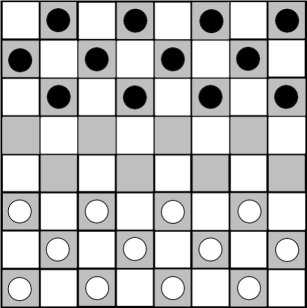
\includegraphics[scale=0.35]{The-starting-position-for-checkers.png}
        \caption{An image showing the starting position of a game of draughts}
    \end{wrapfigure}

    The pieces only move diagonally (so will always be on black squares)
    and the aim is to take all of the opposing players pieces, or to put the opposing player in a position with no possible moves.
    Players take turns moving their shade of pieces. If at any point of the game, a player's piece reaches the opposing players edge
    of the board, the piece becomes a 'King', and another piece should be placed on top of said piece to indicate so.

    Unless a piece is crowned and a 'King' it may only move and take pieces diagonally forwards. Kings may move and take both forwards and backwards.

    If an adjacent square has an opponents piece and the square immediately beyond the oppositions piece is empty, the opponents piece may be captured.
    If the player who's go it is has the opportunity to capture one or more pieces, then they must do so. 
    A piece is taken by moving your own piece over the opposing player's, into the vacant square, and then removing the opposing piece from the board.
    An example of this process can be seen in Figure 2.

    \begin{figure}[h]
        \centering
        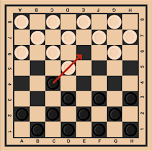
\includegraphics[scale=1.15]{piece being taken.png}
        \caption{Example of a piece being taken in draughts}
    \end{figure}

    Unlike a regular move, a capturing move may make more than one 'hop'. This is if the capture places the piece in a position where another capture.
    In this case, the additional capture must be made. An example of this successive capturing behaviour can be seen in Figure 3. 
    
    \begin{figure}[h]
        \centering
        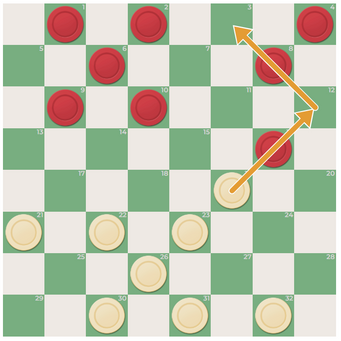
\includegraphics[scale=0.8]{double hop.png}
        \caption{Visualization of a double hop capture}
    \end{figure}

    The move may only end when the position has no more captures available or an uncrowned piece reaches the opposing edge
    of the board and becomes a King. The capture sequence can only be made by one piece per move. I.E. You cannot make on capture with one piece, and then another capture with another piece in the same move.

    However, if more than one piece can capture, the player has free choice over which piece to move. Likewise, if one piece can capture in multiple
    directions then the player has the choice in which direction to move. \textbf{Note:} it is not compulsary for the player to move in the direction, or with the piece,
    that will lead to the greatest number of captures in that move.

    If no capturing moves can be made, then any piece may be moved diagonally onto a vacant square.

    The game ends when all of a players piece's have been captured, or a player has no available moves.

    \subsection{Neural Networks}
    \noindent \url{https://www.ibm.com/topics/neural-networks}

    \subsubsection{What is a neural network}
    A neural network is a machine learning model which aims to mimic the processes of the human brain.
    Each network contains inputs and outputs, as well as one or more layers of hidden nodes - which act as artificial neurons.
    In a fully connected network, each node is connected once to each node in the next layer - an example of how one node connects
    to the next layer can be seen in Figure 4.
    \begin{figure}[h]
        \centering
        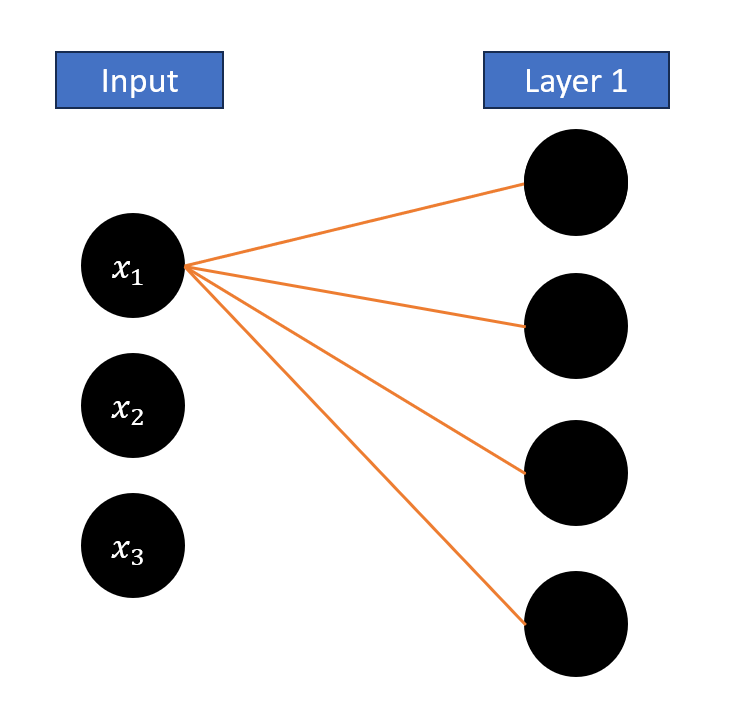
\includegraphics[scale=0.2]{ConnectedNode.png}
        \caption{Example of a fully connected node and layer}
    \end{figure}

    Neural networks are a supervised learning model, meaning that they learn from labeled data (which has the objective correct answer in the data).
    They are sometimes referred to as artificial neural networks (ANNs) or simulated neural networks (SNNs).\\

    Neural networks can be modelled as a collection linear regression units.

    \subsubsection{Linear Regression Unit}
    A single linear regression unit output has the formula:
    \begin{displaymath}
        \hat{y} = \sum_{i=0}^{n} w_ix_i + b
    \end{displaymath}

    Where $\hat{y}$ is the predicted output, $n$ is the number of inputs, $x_i$ is the $i$th input, $w_i$ is the weight of $x_i$, and $b$ is a bias.
    If, for example, there were 3 inputs the full equation for $\hat{y}$ would be:
    \begin{displaymath}
        \hat{y} = w_1x_1 + w_2x_2 + w_3x_3 + b
    \end{displaymath}

    \subsubsection{Vectorization of summations}
    \noindent \url{https://courses.cs.washington.edu/courses/cse446/20wi/Lecture8/08_Regularization.pdf}

    This calculation can be vectorized to improve efficiency and would be notated:
    \begin{displaymath}
        \hat{y} = XW + b
    \end{displaymath}

    Where we let
    \begin{displaymath}
        W = \begin{bmatrix}
            w_1\\
            w_2\\
            \vdots\\
            w_n
        \end{bmatrix}\\
        \hspace{25px}
        X = \begin{bmatrix}
            x_1&
            x_2&
            \hdots&
            x_n
        \end{bmatrix}
    \end{displaymath}

    $X$ here is a row vector as this is the most common format for data as an input to a network (e.g being read from a csv).
    This computation is much faster, and can be parallelized using the GPU to further improve speed and efficiency.

    \subsubsection{Forward Pass of Dense Layer}
    In the case of neural networks, lots of these linear regression units can be combined to form a vector of outputs.
    Each of these regression units will have the same inputs, therefore $X$ can have the same definition. However, $W$ will now be
    composed of multiple vectors of weights, instead of just one.

    Here we let
    \begin{displaymath}
        W = \begin{bmatrix}
            w_11 & w_21 & \dots & w_j1\\
            w_12 & w_22 & \dots & w_j2\\
            \vdots & \vdots & \ddots & \vdots\\
            w_1n & w_2n & \dots & w_jn
        \end{bmatrix}
    \end{displaymath}

    Where $j$ is now the number of nodes in the layer. If we rewrite our forward pass equation to use this weight matrix,
    with each node as its own regression unit:
    \begin{displaymath}
        \begin{bmatrix}
            \hat{y_1}&
            \hat{y_2}&
            \hdots&
            \hat{y_n}
        \end{bmatrix} = \begin{bmatrix}
            x_1&
            x_2&
            \hdots&
            x_n
        \end{bmatrix} \begin{bmatrix}
            w_11 & w_21 & \dots & w_j1\\
            w_12 & w_22 & \dots & w_j2\\
            \vdots & \vdots & \ddots & \vdots\\
            w_1n & w_2n & \dots & w_jn
        \end{bmatrix} + \begin{bmatrix}
           b_1 & b_2 & \dots & b_3
        \end{bmatrix}
    \end{displaymath}


    Again using capital letters to simplify notation, the foward pass through a dense layer looks as follows:
    \begin{displaymath}
        Y = XW + B
    \end{displaymath}

    \subsubsection{Backwards Pass of Dense Layer}
    Although back propogation can be solved in closed form, it comes with a large time complexity (greater than $O(n^3$)), and therefore
    a process called gradient descent is usually employed.


    \pagebreak
    \noindent \url{https://www.turing.com/kb/mathematical-formulation-of-feed-forward-neural-network} Maths?

    \noindent \url{https://en.wikipedia.org/wiki/Automatic_differentiation} Automatic differentiation
\end{document}